\documentclass[10pt,twocolumn,letterpaper]{article}
%% Welcome to Overleaf!
%% If this is your first time using LaTeX, it might be worth going through this brief presentation:
%% https://www.overleaf.com/latex/learn/free-online-introduction-to-latex-part-1

%% Researchers have been using LaTeX for decades to typeset their papers, producing beautiful, crisp documents in the process. By learning LaTeX, you are effectively following in their footsteps, and learning a highly valuable skill!

%% The \usepackage commands below can be thought of as analogous to importing libraries into Python, for instance. We've pre-formatted this for you, so you can skip right ahead to the title below.

%% Language and font encodings
\usepackage[english]{babel}
\usepackage[utf8x]{inputenc}
\usepackage[T1]{fontenc}

%% Sets page size and margins
\usepackage[a4paper,top=2cm,bottom=2cm,left=3cm,right=3cm,marginparwidth=1.75cm]{geometry}

%% Useful packages
\usepackage{amsmath}
\usepackage{graphicx}
\usepackage[colorinlistoftodos]{todonotes}
\usepackage[colorlinks=true, allcolors=blue]{hyperref}
\usepackage{natbib}
\bibliographystyle{unsrt}
%% Title
\title{
		\usefont{OT1}{bch}{b}{n}
		\normalfont \normalsize \textsc{Electronics and Computer Science A10 Report} \\ [10pt]
		\huge Chaotic Harmonics: Inductor-Diode Dynamics \\
}
\selectlanguage{english}
\usepackage{authblk}
\author[1]{kaicho}
\affil[1]{University of Southampton}

\setlength {\marginparwidth }{2cm}
\begin{document}
\maketitle

%%\begin{abstract}
%%This paper aims to present the experimental observations and possible explanations of Inductor-Diode Oscillator dynamics, along with the means used to create and observe these behaviours.  The initial preconceptions of the investigation were only built upon a brief understanding of Capacitor-Diode peak detectors and as such lead to a novel understanding of the chaotic dynamics that the experiment was outlined to entail.  
%%\end{abstract} \\ 
%%\\ 
%%{\textbf{Keywords} \\
%%Stochastic LD Dynamics, Oscillator, Bifurcation, Experimental Feigenbaum Calculation}

\section{Background}
To understand the nature of the findings, it is important to build a brief understanding of chaotic systems and their relationships to this experiment.

Appearing stochastic when observed only by its outcomes, deterministic chaos is a phenomenon which can be observed in systems in which otherwise seemingly insignificant changes in the initial system conditions can have very significant changes to the final observed behaviour.  However, if the entire system is known and accurately modelled, it is possible to accurately \textit{predict} the outcome each minor change will have - hence the behaviour is, unlike true randomness, \textit{deterministic}.  

A conceptually simple example is that of a ball placed on top of a dome.  Assuming all frictional forces to be zero, such a model will result in the ball drastically accelerating in any direction on the \(x\)-\(y\) plane - this large acceleration as a result of the initial position on top of the dome.  Even placing the ball mere picometres off the central axis will result in the ball's acceleration into a determinable direction.

In the case of this experiment, the seemingly random dynamics that arise from minute system changes are that of the frequency of the output waveform as a function of the frequency and amplitude of the input waveform.  Through incrementing an input variable at a constant gradient, we can observe qualitative changes to the output, caused by the chaotic nature of the system.  These qualitative changes are \textit{bifurcations}.  A \textit{bifurcation diagram} can be graphed which shows enclosed regions of values of the input variables that result in the aforementioned \textit{n}-order bifurcations.  An LD system will have a resonant frequency by the nature of the Inductor's dynamics, hence when that frequency or its harmonics are reached, constructive interference will be observed, causing the amplitude to rise to infinity.  It is by taking this resonant frequency as an \textit{asymptote to chaos} that a limited range is created within which the number of bifurcations will tend to infinity.  As a result, the bifurcation diagram with the forward biased resonant frequency as the upper \(x\) asymptote creates a fractal - as magnifying into the asymptote with greater and greater resolution only shows more and more self-similar period doubling bifurcations:- however, it must be noted that in this scenario, that the systems instantaneous resonant frequency is adjusted through adjusting the amplitude of the input waveform\cite{diodefact}.

However, to cause the sudden \textit{qualitative} changes to the output, non-linearity is required\cite{werner1}.  This non-linearity is provided through the intrinsic properties of \textit{Zener} diodes, which will be discussed towards the end of the paper.

\begin{figure}[h]
  \centering
  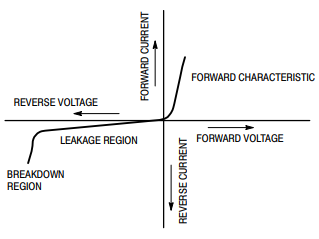
\includegraphics[width=0.4\textwidth]{figures/zener2.png}
  \caption{The non-linear I-V characteristics of a Zener diode, designed to allow for reverse bias operation without damaging the component\cite{diode}.}
\end{figure}

The accuracy of the experiment will be explored through an attempted calculation of the Feigenbaum constant, a value given by the formula:
\[\delta = \lim_{n \to \infty }\frac{\alpha_{n-1} - \alpha_{n-2} }{\alpha_{n} - \alpha_{n-1}} = 4.669...\]
where \(\alpha\) represents the value of bifurcation with subscript representing the order of bifurcations passed\cite{feigenbaum}.  As the number of bifurcations tends to infinity, the ratio of the values of bifurcation for any chaotic system tends towards the \emph{Feigenbaum Constant}.


\section{Experimental Method}

The basic circuit layout for this experiment was very simple, as it only requires the use of two passive components in series:  A 10mH Inductor and a Zener diode. 

An AC voltage source with a maximum \(V_{pk-pk}\) of 20V was connected in series with the circuit alongside a 10x oscilloscope probe CH2 across the voltage source.  Another 10x oscilloscope probe CH1 was connected across the Zener diode.  As the system is very sensitive it is important to use high-impedance probes that will only minimally affect the dynamics.

\begin{figure}[h]
  \centering
  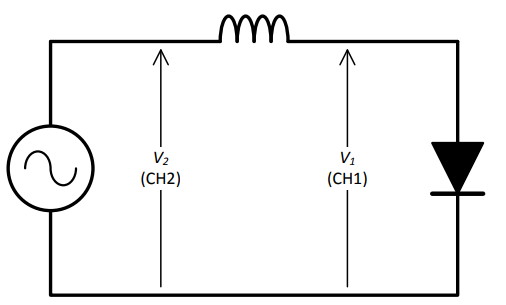
\includegraphics[width=0.4\textwidth]{figures/lab.png}
  \caption{Circuit diagram for the chaotic Inductor-Diode oscillator.}
\end{figure}

To avoid resonance causing out-of-range readings, the AC voltage source was initially set to output a  200m\(V_{pk-pk}\) sine wave at a frequency, \(f\), of 180kHz.  Afterwards, the frequency is slowly incremented until the resonant frequency \(f_{resonance}\) is found.  This value will vary; however, this experiment found \(f_{resonance}\) to stabilise at 211.4kHz.

Once \(f_{resonance}\) has been identified, \(f\) must be adjusted such that it lies on the verge of resonance. This experiment found \(f\) to be stable at 205kHz.

After \(f\) has been chosen, the AC input \(V_{pk-pk}\) needs to be finely increased.  As the voltage increases steadily, the amplitude of \(V_2\) should increase.  While \(V_2\) is increasing, observe the waveform displayed on \(V_1\).

To thus experimentally calculate the values for \(\alpha_{n}\), the voltage ranges in which bifurcation is observed on the oscilloscope trace \(V_2\) must be measured and calculated to produce an average value and its uncertainty.  These values can then be used in the formula:  
\[\delta = \lim_{n \to \infty }\frac{\alpha_{n-1} - \alpha_{n-2} }{\alpha_{n} - \alpha_{n-1}} = 4.669...\]
to calculate the final Feigenbaum number.
\\
\\
\\

\section{Results}

The results from this experiment showed great variation in the values of bifurcation \(\alpha_n\), with the uncertainty only decreasing after the second bifurcation, \(\alpha_2\), as can be seen in the table below.  \(\alpha_0\) represents the initial voltage for the first bifurcation, hence it does not have a range as the proceeding values of \(\alpha\). 

\begin{table}[h]
\begin{tabular}{|c|cccc|}
\hline
\(\alpha_n\)  & m\(V_{min}\) & m\(V_{max}\) & m\(V_{avg}\) & Uncertainty  \\ \hline
\(\alpha_0\)  & n/a          & n/a          & 251          & n/a          \\
\(\alpha_1\)  & 3016         & 3925         & 3470         & 455          \\
\(\alpha_2\)  & 6435         & 7405         & 6920         & 485          \\ 
\(\alpha_3\)  & 11755        & 11845        & 11800        & 45           \\ \hline
\end{tabular}
\end{table}

Due to the voltage limitations of the AC voltage source, the apparent decreasing trend of the uncertainty could not be investigated any further, thus the calculations of the Feigenbaum number had to be calculated with those uncertainties taken into consideration.

\begin{figure}[h]
  \centering
  \includegraphics[width=0.4\textwidth]{figures/freqh.png}
  \caption{This oscilloscope trace shows trace \(V_1\) after the bifurcation value \(\alpha_2\).}
\end{figure}
\begin{figure}[h]
  \centering
  \includegraphics[width=0.4\textwidth]{figures/image (3).png}
  \caption{This oscilloscope trace shows trace \(V_1\) with a lower frequency after the bifurcation value \(\alpha_3\).  It is important to note the 0V position of the \(V_1\) trace.  There is considerable clipping of the sine wave at the top - clipped to the forward voltage \(V_f\) of the diode.  However, the other important aspect is the much greater negative bias across the diode, at more than -7V.  This becomes important in explaining the behaviour of the circuit.}
\end{figure}

As can be seen in Figures 3 and 4, the frequency does show period doubling bifurcation (although unfortunately due to the time scale this is not apparent at first).  However, as the range of voltages bifurcation was observed, it was difficult to reliably decide which voltage range to use. 

\begin{figure}[h]
  \centering
  \includegraphics[width=0.4\textwidth]{figures/blow.png}
  \caption{This oscilloscope trace shows bifurcation of trace \(V_1\) at the lowest voltage at which bifurcation could be observed.}
\end{figure}
\begin{figure}[h]
  \centering
  \includegraphics[width=0.4\textwidth]{figures/bhigh.png}
  \caption{This oscilloscope trace shows bifurcation of trace \(V_1\) at the highest voltage at which bifurcation could be observed.}
\end{figure}

Thus, using these values, a experimental value for the Feigenbaum constant can be calculated as follows:

\[\delta = \frac{3450 \pm 940}{4880 \pm 530} = \frac{3450 \pm 27.2\%}{4880 \pm 10.9\%}\]
\[\delta = 0.707 \pm 38.1\%\]

The experimental value calculated is in excess of 5 times smaller than the actual Feigenbaum constant.  The reasoning for which is most likely due to a multitude of reasons, however, the formula for calculating the Feigenbaum is a limit and is only completely valid when the number of bifurcations measured tends to infinity.  As we can only experimentally measure the first few values of bifurcation it is not entirely surprising the value calculated was not accurate.

\section{Discussion}
Fortunately, despite being unable to produce a value consistent with the accepted Feigenbaum number, the results observed allow for many of the previously made postulates to be drawn together into a hypothesis regarding the chaotic nature of the LD circuit. 

\textbf{\textit{Hypothesis:}} As previously mentioned in \textit{Figure 1} the Zener Diode carries interesting IV characteristics that allow it to safely conduct and \textit{clamp} voltage in both the positive and negative bias.  However, it was also mentioned that the resonant frequency of the circuit was being modified by the input waveform amplitude - the changing voltage across the diode.  
This is possible due to a phenomenon seen in P-N junctions.  When operating in the reverse bias, P-N junction diodes such as Zener diodes initially act as capacitors as the increasing depletion zone creates two saturated P-type and N-type conductors, allowing for high conductivity either side of the diode while leaving an insulating dielectric in between\cite{diodefact}.  Recall from \textit{Figure 4} that the reverse voltage clamp in the was seen to drop as low as -7 volts. 
Recall that the resonance frequency \(f_{resonance}\) is given by the formula:
\[f_{resonance} = \frac{1}{2\pi\sqrt{LC}}\]
The value of C scales inversely with the magnitude of the reverse voltage across the diode as the depletion zone widens due to the voltage\cite{diodefact} as:
\[C = \frac{\varepsilon A}{d}\]
This has the effect of increasing \(f_{resonance}\) \textbf{only} on the \textbf{negative} cycle of the sine wave causes the voltage to rise again sharply, creating the stable output waveform that appears to be a fully rectified sine wave clamped to \(V_f\) and \(V_{rev}\) seen in \textit{Figure 4}.
\begin{figure}[h]
  \centering
  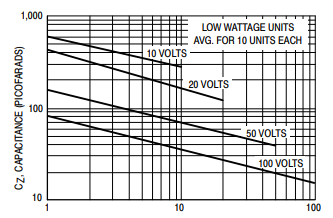
\includegraphics[width=0.4\textwidth]{figures/revcap.png}
  \caption{As \(V_{rev}\) increases from 0 to -10v, capacitance halves\cite{revcap}.}
\end{figure}

The next two Figures, 8 and 9, demonstrate how \(V_{rev}\) affects the frequency of \(V_1\).  \textit{Figure 8} shows a much lower \(V_{rev}\) of 0.9V, whereas \textit{Figure 9} shows a higher \(V_{rev}\) of 7.5V.  As such the peak is much sharper relative to their corresponding input waves.
\begin{figure}[h]
  \centering
  \includegraphics[width=0.4\textwidth]{figures/wide.png}
  \caption{Observe the width of the reverse peak compared to the input wave.}
\end{figure}
\begin{figure}[h]
  \centering
  \includegraphics[width=0.4\textwidth]{figures/image (3).png}
  \caption{Observe the width of the reverse peak compared to the input wave.}
\end{figure}
\\
This still, albeit, does not explain the chaotic behaviour, or the behaviour on the positive cycle of the sine wave.  However; on the positive cycle, despite having no significant capacitance, the effects of the capacitive behaviour remain, and become more pronounced as the magnitude of the voltage \textit{increases}.  

Similar to how the capacitance between a Field-Effect Transistor's Gate and Drain-Source limits its switching speed, the previously mentioned reverse-bias capacitance also affects the switching speed of the \textit{diode}.  

Previously it was emphasised that the increase of \(f_{resonance}\) was very \textbf{brief} and proportional to the reverse voltage spikes.  This is because in actuality, as the voltage increases, the \textbf{net} parasitic capacitance \textit{increases}. However, rather than a capacitance that arises as a result of an electric field across a dielectric, this parasitic capacitance is a result of the physical \textit{charge carriers} within the silicon travelling a distance away from their initial position which is proportional to the voltage applied across the junction.  Thus, as \(V_{pk-pk}\) increases, the switching time from each bias \(t_s\) also increases\cite{switching}.  This leads to the second aspect of the hypothesis.  

Modifying the metaphoric ball on a dome analogy, replacing the dome with a series of \textit{hills and valleys} along the frequency domain, the bottom of each valley can be thought of as a \textit{harmonic} of the \textit{natural resonant frequency} - i.e. 
\[f_{n} = {2^{n}}{f_{resonance}}\]
As the number of hills and valleys increase, the spacing between them increases, and their steepness decreases.  
As the value of bifurcation, \(V_{pk-pk}\) increases, \(t_s\) increases.  This causes the ball - the frequency of the circuit - to start being pushed up the hill - pushed out of phase - into an energetically unstable position. This is what is observed when the waveform begins to split and become offset from one another in \textit{Figures 5 and 6}.  Eventually, \(V_{pk-pk}\) increases past the point where \(t_s\) causes the ball to roll over the top of the hill and collapse into a lower harmonic, a stable energy state: - the sudden, qualitative change observed from a gradual, constant change in the value of bifurcation.

Leaving the analogy, it should be noted that the actual operation is more complicated, as, this means that the \textit{net} capacitance is constantly changing with time as not only is it changing on the negative cycle due to the depletion zone but also on the positive cycle when the switching delay causes the diode to start missing cycles.  The result of this changing capacitance is most likely what causes the complex superposition of waveforms observed between bifurcations such as that seen in \textit{Figure 5}.  Alas too complicated for a first year to even start to try to understand.

\section*{Bibliography}
\begin{thebibliography}{9}

\bibitem[1]{diodefact}
ON Semiconductor, (2017), \emph{Zener Theory and Design Considerations}, Published by SCILLC, Handbook HBD854/D 1st. Edition pp.25-26 

\bibitem[2]{werner1}
Rheinboldt, Werner C.  \emph{Nonlinear Systems and Bifurcations∗}, University of Pittsburgh.

\bibitem[3]{diode}
ON Semiconductor, (2017), \emph{Zener Theory and Design Considerations}, Published by SCILLC, Handbook HBD854/D 1st. Edition pp.19 Figure 1

\bibitem[4]{feigenbaum}
Weisstein, Eric W. \emph{Feigenbaum Constant.} https://mathworld.wolfram.com

\bibitem[5]{revcap}
ON Semiconductor, (2017), \emph{FREQUENCY AND PULSE CHARACTERISTICS}, Published by SCILLC, Handbook HBD854/D 1st. Edition pp.26 Figure 22

\bibitem[6]{switching}
ON Semiconductor, (2017), \emph{HIGH FREQUENCY AND SWITCHING
CONSIDERATIONS}, Published by SCILLC, Handbook HBD854/D 1st. Edition pp.28

\end{thebibliography}
\end{document}
